\documentclass[tikz,border=5mm]{standalone}
\usepackage[T1]{fontenc}
\usepackage{fontspec}
\setmainfont{Fira Sans}[
  BoldFont=Fira Sans Bold,
  ItalicFont=Fira Sans Italic,
]
\usetikzlibrary{positioning, arrows.meta, shadows.blur, calc, decorations.pathmorphing}

\definecolor{mTeal}{HTML}{2B7A78}
\definecolor{mBrown}{HTML}{C9956B}
\definecolor{mRed}{HTML}{CC4444}
\definecolor{mGreen}{HTML}{3A8A3A}
\definecolor{mGray}{HTML}{888888}
\definecolor{mBg}{HTML}{FAFAFA}

\begin{document}
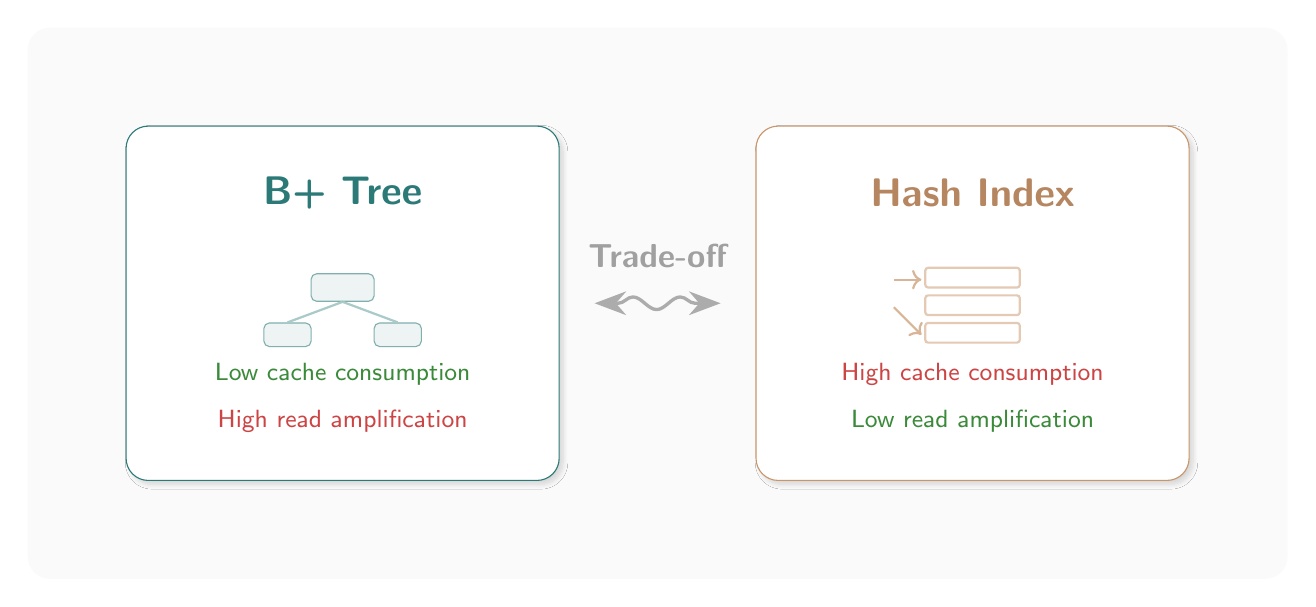
\begin{tikzpicture}[
  every node/.style={font=\sffamily},
]
  % Background
  \fill[mBg, rounded corners=8pt] (-8,-3.5) rectangle (8,3.5);

  % B+ Tree box
  \node[draw=mTeal, fill=white, rounded corners=8pt, minimum width=5.5cm,
        minimum height=4.5cm, blur shadow={shadow blur steps=8, shadow xshift=0.5mm,
        shadow yshift=-0.5mm, shadow opacity=15}] (btree) at (-4,0) {};
  \node[font=\sffamily\Large\bfseries, mTeal] at (-4, 1.4) {B+ Tree};
  % Tree icon
  \begin{scope}[shift={(-4,0.2)}]
    \node[draw=mTeal!60, fill=mTeal!8, rounded corners=2pt, minimum width=0.8cm,
          minimum height=0.35cm, font=\tiny\sffamily] (tr) at (0,0) {};
    \node[draw=mTeal!60, fill=mTeal!8, rounded corners=2pt, minimum width=0.6cm,
          minimum height=0.3cm, font=\tiny\sffamily] (tl) at (-0.7,-0.6) {};
    \node[draw=mTeal!60, fill=mTeal!8, rounded corners=2pt, minimum width=0.6cm,
          minimum height=0.3cm, font=\tiny\sffamily] (trr) at (0.7,-0.6) {};
    \draw[mTeal!40, thick] (tr.south) -- (tl.north);
    \draw[mTeal!40, thick] (tr.south) -- (trr.north);
  \end{scope}
  \node[mGreen, font=\sffamily\small] at (-4,-0.9) {Low cache consumption};
  \node[mRed, font=\sffamily\small] at (-4,-1.5) {High read amplification};

  % Hash Index box
  \node[draw=mBrown, fill=white, rounded corners=8pt, minimum width=5.5cm,
        minimum height=4.5cm, blur shadow={shadow blur steps=8, shadow xshift=0.5mm,
        shadow yshift=-0.5mm, shadow opacity=15}] (hash) at (4,0) {};
  \node[font=\sffamily\Large\bfseries, mBrown!90!black] at (4, 1.4) {Hash Index};
  % Hash icon
  \begin{scope}[shift={(4,0.2)}]
    \foreach \y in {0, -0.35, -0.7} {
      \draw[mBrown!50, thick, rounded corners=1pt] (-0.6,\y) rectangle (0.6,\y+0.25);
    }
    \draw[mBrown!70, ->, thick] (-1,0.1) -- (-0.65,0.1);
    \draw[mBrown!70, ->, thick] (-1,-0.25) -- (-0.65,-0.6);
  \end{scope}
  \node[mRed, font=\sffamily\small] at (4,-0.9) {High cache consumption};
  \node[mGreen, font=\sffamily\small] at (4,-1.5) {Low read amplification};

  % Trade-off arrow
  \draw[{Stealth[length=4mm, width=3mm]}-{Stealth[length=4mm, width=3mm]},
        very thick, mGray!70, decorate,
        decoration={snake, amplitude=0.8mm, segment length=6mm, post length=3mm, pre length=3mm}]
    (-0.8,0) -- (0.8,0);
  \node[font=\sffamily\bfseries\large, mGray!80, fill=mBg, inner sep=3pt] at (0,0.6) {Trade-off};
\end{tikzpicture}
\end{document}
